\section{Theory}
Identical infinitely-long thin metal plates $A_1,A_2,A_3,A_4,A_5,B_1,B_2,B_3 $ and $B_4$ are placed in an \textit{interleaved} arrangement as dipicted in fig1.(a) Group of plates $A_i$ and $B_i$ are connected to the terminal $A$ and $B$ , respectively, by means of gold wires. The terminals are connected to different potential sources $U_A$ and $U_B$ respectively. \\
This is called an interleaved capacitor, Our goal will be to approximate the potential distribution (in two dimensions considering symmetry along the the third axis which will be dropped) inside the capacitor after we disconnect the capacitor from sources, treating the interior plates as line charge distributions.
\begin{align*}
    &U_A = 5V \\
    &U_B = -5V \\
    &\text{Capacitance } = 0.1\mu F\\
    &\text{Distance between plates ($d$)} = 0.5\mu m \\
    &\textit{Dimensions: } 4 \times 4.4 \mu m  
\end{align*}
This arrangement can be seen as a number of parallel plate capacitors connected in parallel to each other as seen in fig1(b),
if $C_0$ is the capacitance of each capacitor in parallel and $C$ is the capacitance of the entire arrangement then,
\begin{align*}
    C_0 = C/8
\end{align*}
Also we know that for parallel plate capacitors with cross-section area $A$ and distance $d$ between the plates,
\begin{align}
    C_0 = \epsilon_0 \frac{A}{d} \implies A = \frac{C_0d}{\epsilon_0}
\end{align}
Therefore the charge distribution on any plate $A_i$ is given by,
\begin{align}
    \rho_A = \frac{(C \times V )}{5A} \implies \rho_A = 2\epsilon_0 \times 10^5C m^{-2} 
\end{align}
Similarly on $B_i$,
\begin{align}
    \rho_B = -2\epsilon_0 \times 10^5C m^{-2} 
\end{align}

\begin{figure}[h]
    \centering
    \begin{subfigure}[b]{\linewidth}
    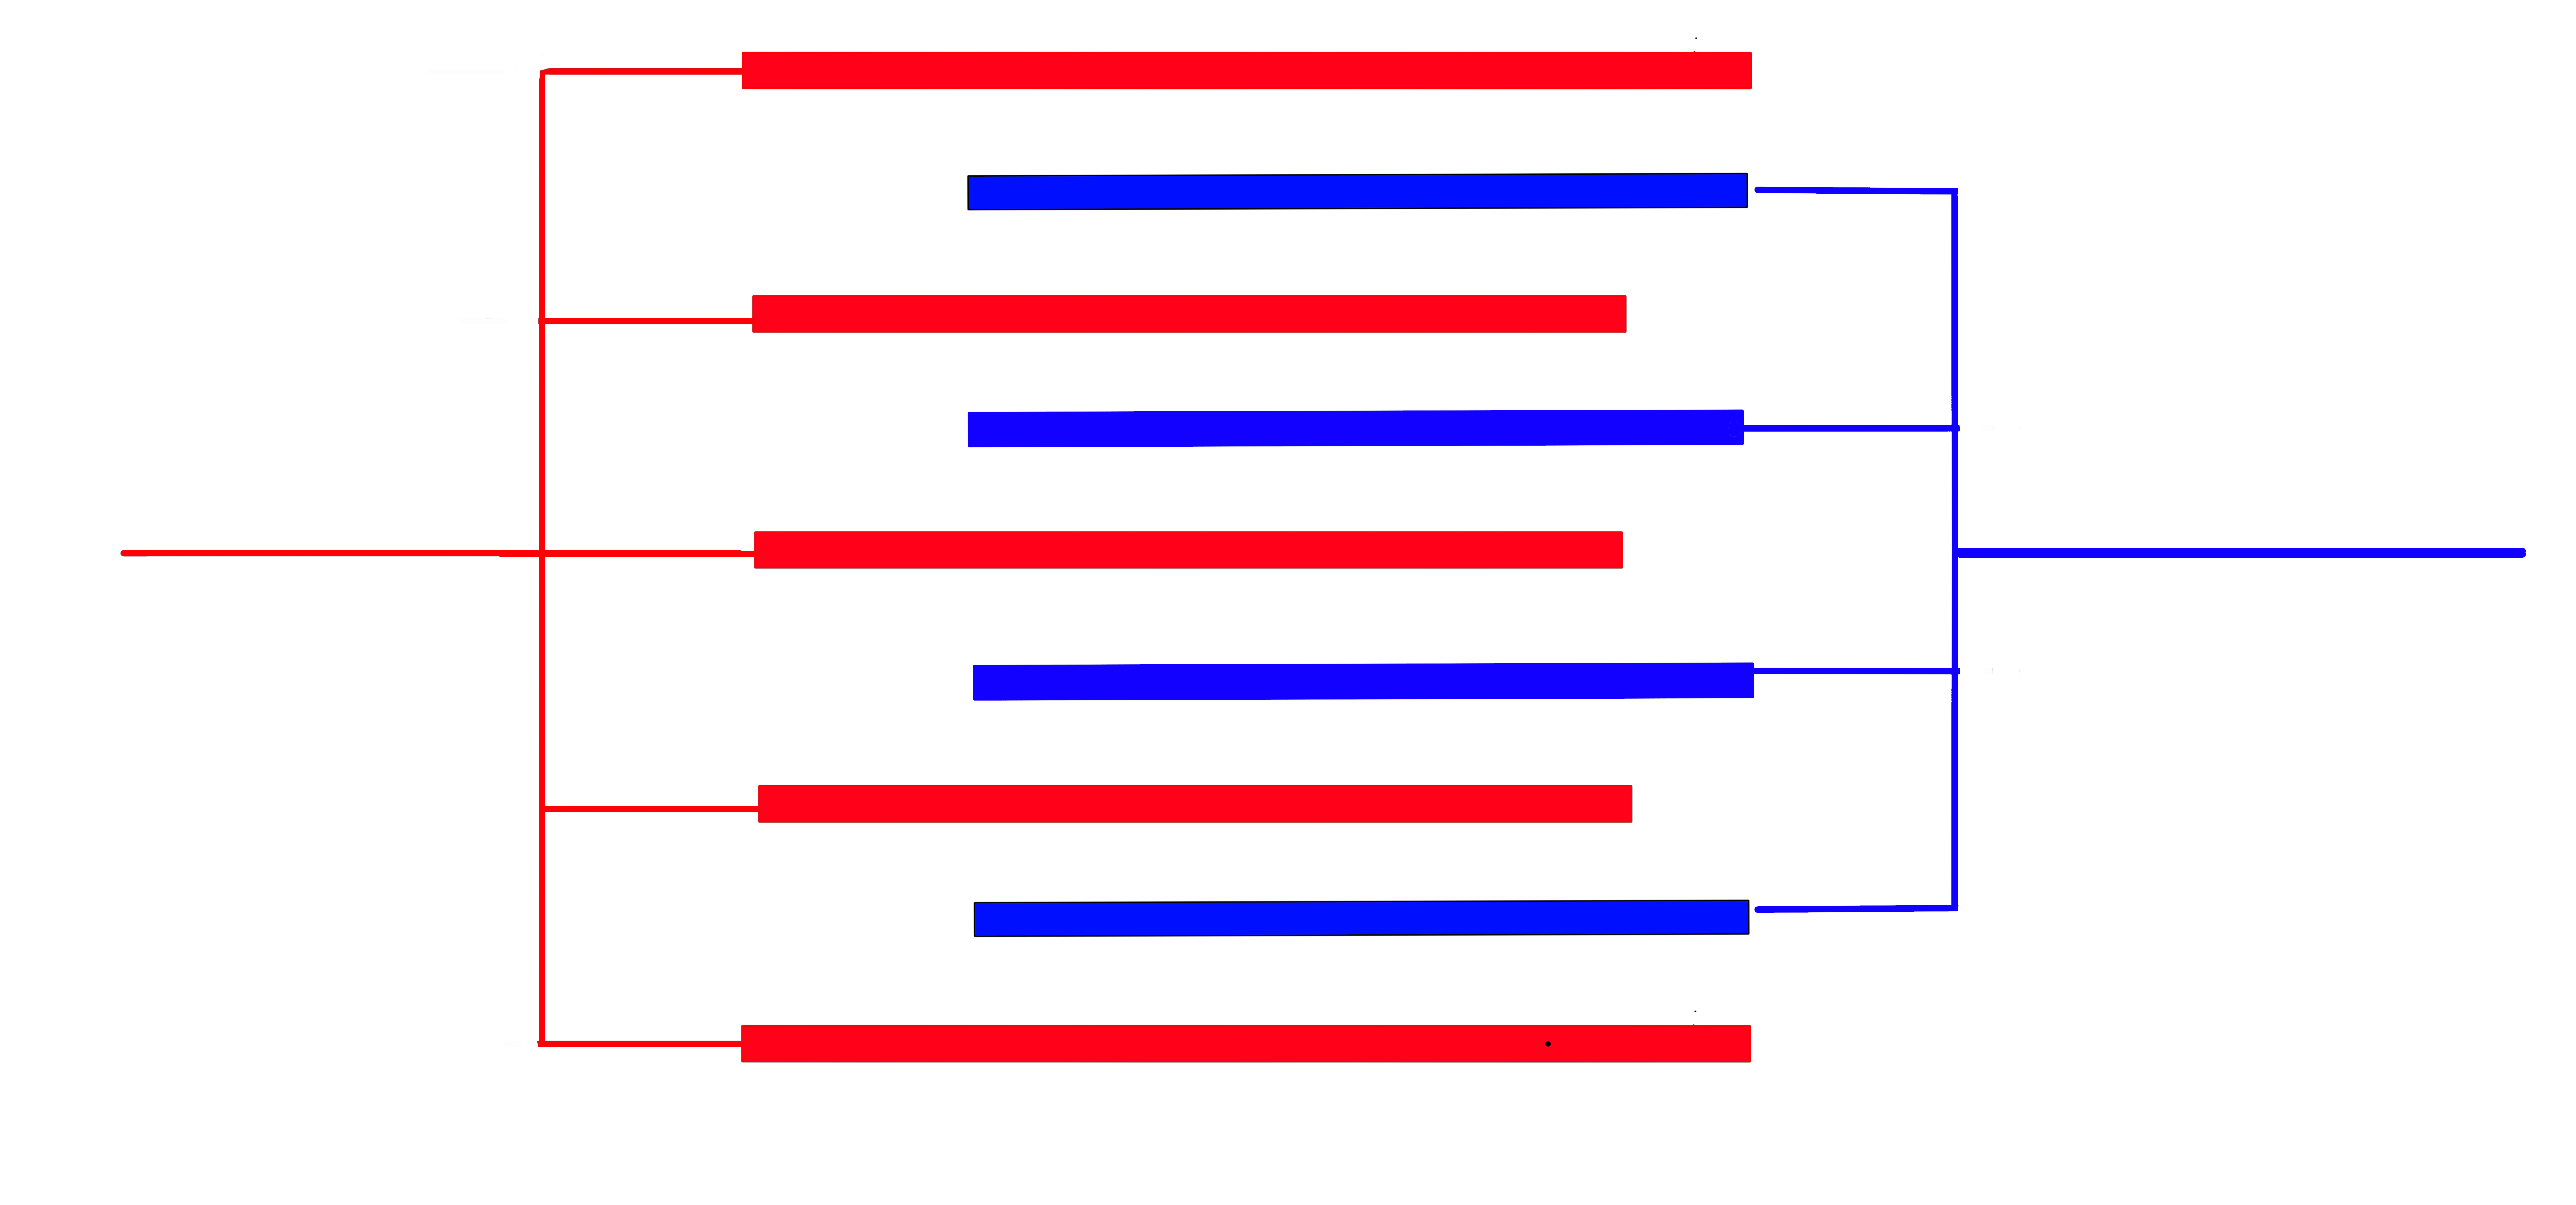
\includegraphics[width=5cm, height=4cm]{content/capacitor.png}
    \caption{\small Diagram dipciting the arrangement of plates in a interleaved fashion.}
    \label{fig 1: the capacitor}
    \end{subfigure}
\end{figure}
Mathematical Formulation:\\
Let $U(x,y)$ and $\vec{E}(x,y)$ be the potential and Electric field distribution defined in the region of our arrangement $(x,y) = [0,4\mu m]\times[0,4.4\mu m]$ .\\
We know from maxwell's laws that for static electric fields $\vec{\nabla} \cdot \vec{E} = \rho / \epsilon_0 $, $\vec{\nabla} \times \vec{E} = 0$
\\
From the later we get $E=-\vec{\nabla}U$, substituting this back into the former we get,
\begin{equation*}
    \vec{\nabla}^2 U = \frac{-\rho}{\epsilon_0}  
\end{equation*}
In two dimensions with euclidean coordinate system the equation reduces to, 
\begin{equation}
    \frac{\pa^2U(x,y) }{\pa x^{2}} + \frac{\pa^2U(x,y) }{\pa y^{2}}= -\frac{\rho(x,y)}{\epsilon_0} \\
\end{equation}
where,
\begin{equation}
\rho(x,y) =  \begin{cases}
    -2\epsilon_0 \times 10^5 C m^{-2} & :\text{if} \gs (x,y) \in B_i \gs \text{where} \gs i = 1,2,3,4 \\
    2\epsilon_0 \times 10^5 C m^{-2} & :\text{if} \gs (x,y) \in A_i \gs \text{where} \gs i = 2,3,4  \\
    0 C m^{-2} & : \gs \text{elsewhere} \\
\end{cases}  
\end{equation}
Now according to our given arrangement,
\begin{align}
    B_1 &= \{ (x^*,y^*) \gs : \gs x^*= 0.5\mu m \gs;\gs 0.4\mu m \leq y^* \leq 4.4\mu m \} \\
    B_2 &= \{ (x^*,y^*) \gs : \gs x^*= 1.5\mu m \gs;\gs 0.4\mu m \leq y^* \leq 4.4\mu m \} \\
    B_3 &= \{ (x^*,y^*) \gs : \gs x^*= 2.5\mu m \gs;\gs 0.4\mu m \leq y^* \leq 4.4\mu m \} \\
    B_4 &= \{ (x^*,y^*) \gs : \gs x^*= 3.5\mu m \gs;\gs 0.4\mu m \leq y^* \leq 4.4\mu m \} \\
    A_2 &= \{ (x^*,y^*) \gs : \gs x^*= 1\mu m \gs;\gs 0\mu m \leq y^* \leq 4\mu m \} \\
    A_3 &= \{ (x^*,y^*) \gs : \gs x^*= 2\mu m \gs;\gs 0\mu m \leq y^* \leq 4\mu m \} \\
    A_4 &= \{ (x^*,y^*) \gs : \gs x^*= 3\mu m \gs;\gs 0\mu m \leq y^* \leq 4\mu m \} 
\end{align}
We get the following boundary conditions for the above boundary value problem,
\begin{align}
    & U(0,y) = +5 V \gs; \gs U(4,y) = +5 V \\ 
    & U_y(x,0) = 0V/m \gs; \gs U_y(x,4.4) = 0V/m 
\end{align}

Non-Dimensionalizing the variables,

Let new dimensionless variables,
\begin{align}
    x' = \frac{x}{s} \gs \gs y' = \frac{y}{s} \gs \gs U' = \frac{U}{\nu}
\end{align}
where $s$ and $\nu$ are known constant scaling factors having dimensions of length and electric potential respectively.

The B.V.P reduces to,
\begin{equation}
    \frac{\pa^2U'(x',y') }{\pa x^{'2}} + \frac{\pa^2U'(x',y') }{\pa y^{'2}}= -\frac{\rho'(x',y') s^2}{\epsilon_0 \nu} \\
\end{equation}
where,
\begin{equation}
\rho'(x',y') =  \begin{cases}
    -2\epsilon_0 \times 10^5  & :\text{if} \gs (x',y') \in B_i \gs \text{where} \gs i = 1,2,3,4 \\
    2\epsilon_0 \times 10^5 & :\text{if} \gs (x',y') \in A_i \gs \text{where} \gs i = 2,3,4 \\
    0  & : \gs \text{elsewhere} \\
\end{cases}
\end{equation}
Now according to our given arrangement,
\begin{align}
    B_1 &= \{ (x^*,y^*) \gs : \gs x^*= 0.5/s \gs;\gs 0.4/s \leq y^* \leq 4.4/s \} \\
    B_2 &= \{ (x^*,y^*) \gs : \gs x^*= 1.5/s \gs;\gs 0.4/s \leq y^* \leq 4.4/s \} \\
    B_3 &= \{ (x^*,y^*) \gs : \gs x^*= 2.5/s \gs;\gs 0.4/s \leq y^* \leq 4.4/s \} \\
    B_4 &= \{ (x^*,y^*) \gs : \gs x^*= 3.5/s \gs;\gs 0.4/s \leq y^* \leq 4.4/s \} \\
    A_2 &= \{ (x^*,y^*) \gs : \gs x^*= 1/s \gs;\gs 0/s \leq y^* \leq 4/s \} \\
    A_3 &= \{ (x^*,y^*) \gs : \gs x^*= 2/s \gs;\gs 0/s \leq y^* \leq 4/s \} \\
    A_4 &= \{ (x^*,y^*) \gs : \gs x^*= 3/s \gs;\gs 0/s \leq y^* \leq 4/s \} 
\end{align}
We get the following boundary conditions for the above boundary value problem,
\begin{align}
    & U(0,y) = +5/\nu \gs; \gs U(4,y) = +5/\nu \\ 
    & U_y(x,0) = 0 \gs; \gs U_y(x,4.4) = 0 
\end{align}

%%%%%%%%%%%%%%%END%%%%%%%%%%%%%%%%%%%%%%